\section{Knowledge Graph Contrastive Fusion}

In this section, we will introduce our proposed ConFu method for PSR task with KG. Figure \ref{kgconfu} is the overview of ConFu, which adopts a two-tower architecture for faster retrieval and ranking in real-time search. Different from previous knowledge fusion methods, ConFu uses contrastive learning to inject knowledge from KG into the model during fine-tuning stage. ConFu is a multi-task learning framework and there are three tasks: one classification task, one query contrastive learning task and one product contrastive learning task. ConFu is based on Sentence-BERT (SBERT) \cite{reimers2019sentence}, which uses a classification objective function during fine-tuning and computes similarity score in the inference stage. Two contrastive learning tasks are designed to inject query-side knowledge and product-side knowledge in KG into the model respectively to help model understand user intent and product essence. 

\begin{figure}[thbp] \centering
    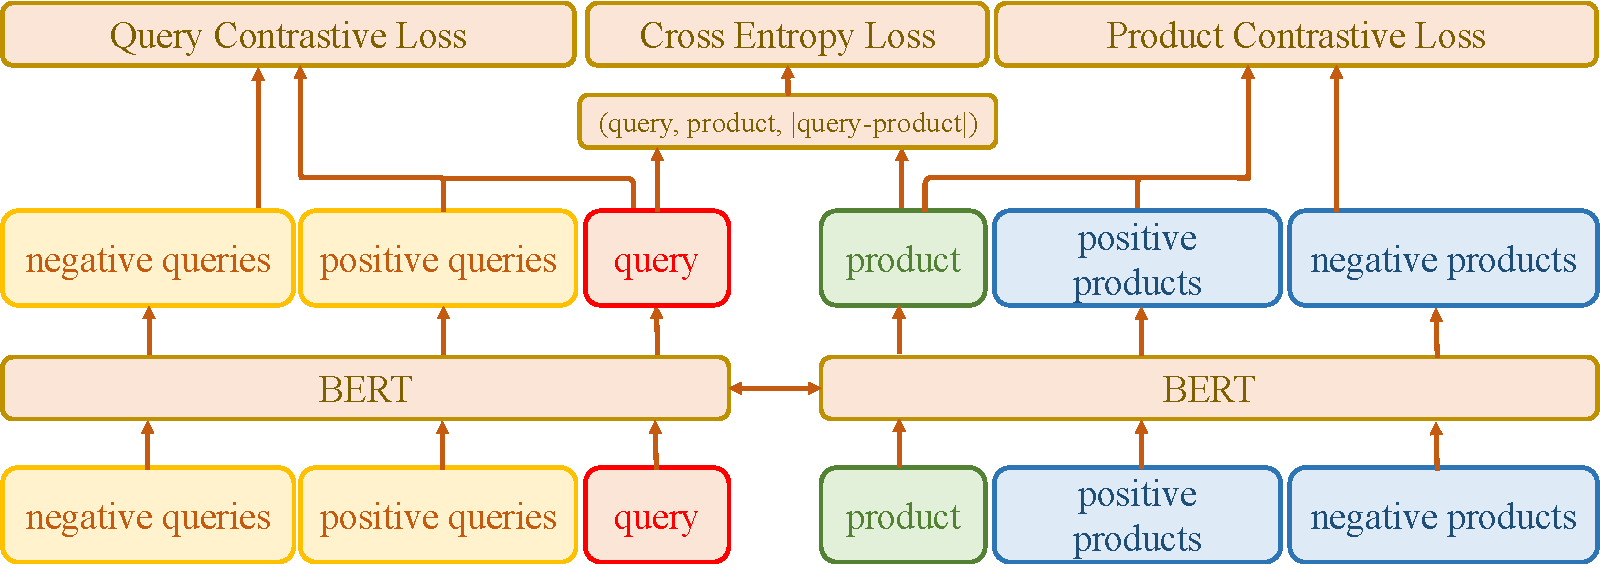
\includegraphics[width=0.48\textwidth]{kgconfu_overview_4}
    \caption{Overview of \textit{ConFu}.}
    \label{kgconfu}
\end{figure}


\subsection{Query Contrastive Knowledge Fusion}
In the query side, we utilize KG to explore positive and negative samples as knowledge for Query Contrastive Knowledge Fusion (QCKF). As a query is usually short and most queries can perform as concepts in KG, the concept graph in KG can be the main source of knowledge for query. The basic idea is that synonyms, hypernyms, hyponyms and other relevant concepts of query can be selected as its positive samples. \xiujie{Irrelevant concepts such as concepts with \textit{irrelevant} relation with the query or other concepts without relation with the query can be selected as negative samples for the query.} With these positive and negative samples, PSR model will be able to learn knowledge behind KG to understand user query better.

% \zelin{what is the `concept net'? is it ConceptNet or the concept graph in dataset? maybe we should emphasize the concept graph and category taxonomy in the begining, otherwise reviewers might be confused here}

% such as synonyms and hypernyms are usually selected as
% we use contrastive learning approach to fuse knowledge into the representation of query.

Specifically, for each query $q$, one positive sample $q_{pos}$ and one negative sample $q_{neg}$ are selected from KG. Other queries in the same batch will be treated as random negative samples. The query contrastive loss is displayed as Equation \ref{qcl}.

% \begin{equation}
%     \begin{aligned}
%     \mathcal{L}^{QCL}&=-{\log\frac{\exp(\mathbf{q}\cdot\mathbf{q}_{pos}/\tau)}{\sum_{k}^{i=1}\frac{\exp(\mathbf{q}\cdot\mathbf{q}_{i}/\tau)}}. 
%     \end{aligned}
% \end{equation}

% \begin{equation}
%     \mathcal{L}^{QCL} = -{\log\frac{\exp(\mathbf{q}\cdot\mathbf{q}_{pos}/\tau)}{\sum_{i=1}^{B} \exp(\mathbf{q}\cdot\mathbf{q}_{i}/\tau)}}
% \end{equation}

\begin{equation}
    \label{qcl}
    \begin{aligned}
    \mathcal{L}_{QCKF}&=-{\log\frac{\exp(\mathbf{q}\cdot\mathbf{q}_{pos}/\tau)}{Q_{Pos}+Q_{Neg}}}. \\
    Q_{Pos}&={\exp(\mathbf{q}\cdot\mathbf{q}_{pos}/\tau)}, \\
    Q_{Neg}&={\exp(\mathbf{q}\cdot\mathbf{q}_{neg}/\tau)} + \sum_{i=1}^{B-1}
    {\exp(\mathbf{q}\cdot\mathbf{q}_{neg, i}/\tau)},\\
    \end{aligned}
\end{equation}

\noindent where $B$ is batch size and $\tau$ is a hyper-parameter for temperature scaling.

The contrastive loss maximizes the similarity between the query $\mathbf{q}$ with its corresponding positive sample $\mathbf{q}_{pos}$. According to the properties of the softmax function, the similarity between the query with those negative samples $\{\mathbf{q}_{neg}, \mathbf{q}_{neg, 1}, \mathbf{q}_{neg, 2}, ..., \mathbf{q}_{neg, B-1}\}$ is minimized.


\subsection{Product Contrastive Knowledge Fusion}
In KG, products are usually organized by a hierarchical taxonomy. Thus, we mainly utilize this taxonomy to generate positive and negative samples for products. Specifically, homonyms are selected as positive samples and products in other categories will be treated as negative samples. With both positive and negative samples sampled from KG, different relationship knowledge and KG structure knowledge can be injected to our model.

Referring to Self-Tuning\cite{wang21}, We adopt Group Contrastive Learning to perform Product Contrastive Knowledge Fusion (PCKF). For each product, we selected a group of positive samples from KG and use products from other groups in the same batch as negative samples. These contrastive groups are arranged in each batch. One advantage of such kind of arrangement \xiujie{compared with random sampling negative samples} is that there will be no false negative samples given labels (KGPs) are correct.

\begin{equation}
    \begin{aligned}
    \mathcal{L}_{PCKF}&=-\frac{1}{D}\sum_{d=1}^{D}{\log\frac{\exp(\mathbf{p}\cdot\mathbf{p}_{pos,d}/\tau)}{P_{Pos}+P_{Neg}}}. \\
    P_{Pos}&=\sum_{d=1}^{D}{\exp(\mathbf{p}\cdot\mathbf{p}_{pos, d}/\tau)}, \\
    P_{Neg}&=\sum_{i=1}^{B-D}
    {\exp(\mathbf{p}\cdot\mathbf{p}_{neg,i}/\tau)},\\
    \end{aligned}
\end{equation}

\noindent where $D$ is the number of positive samples in a contrastive group, $B$ is batch size, $\tau$ is a hyper-parameter for temperature scaling.

The contrastive loss maximizes the similarity between the product $\mathbf{p}$ with its corresponding positive samples $\{\mathbf{p}_{pos,1}, \mathbf{p}_{pos,2}, ..., \mathbf{p}_{pos,D}\}$. The similarity between the product with those negative samples $\{\mathbf{p}_{neg, 1}, \mathbf{p}_{neg, 2}, ..., \mathbf{p}_{neg, B-D}\}$ is minimized.

\subsection{Partial Multi-task Training Strategy}
For those samples hard to find knowledge to fuse due to long tail effect, instead of throwing away these data, we choose to use a training strategy called Partial Multi-task Training Strategy to keep all data samples. 

In detail, we arrange samples with contrastive knowledge (i.e. positive and negative samples) into contrastive batches and samples without contrastive knowledge into non-contrastive batches. In each contrastive batch, there are several groups of products and each group contains products with the same third category in the taxonomy. For each product in the batch, other products in the same group are taken as its positive samples and products in different groups are negative samples. For each query in the batch, a positive query and negative query is sampled in a supervised manner based on relations in KG. Other queries are taken as unsupervised negative samples for the query. Thus, the overall loss of ConFu for contrastive batches is:
% When there is positive and negative samples for query or product
\begin{equation}
    \begin{aligned}
    L&= L_{CE} + \lambda_q L_{QCKF} + \lambda_p L_{PCKF}, \\
    \end{aligned}
\end{equation}

The non-contrastive batches are just batches of query product pairs without external knowledge to be fused. Thus, for non-contrastive batches, $\lambda_q$ and $\lambda_p$ will be set to zero, which means the loss will be the simplified as traditional Cross Entropy Loss. 

\begin{equation}
    L = L_{CE}
\end{equation}

% Generally speaking, the overall structure of ConFu is displayed in Fig \ref{ConFu}, which follows a bi-tower structure with bi-contrastive learning.